% Chapter 5
\chapter{Advertisement Low fidelity prototype} % Main chapter title

\label{Chapter5} % For referencing the chapter elsewhere, use \ref{Chapter1} 
\newpage


\section{Introduction}
For early application development \emph{Formative studies} are required that would assist in design process of that application, and meanwhile it would investigate usability issues with the application prototypes. \emph{Charles M. Reigeluth} \cite{formativestudy} says ``\emph{Formative evaluation (sometimes called field testing or usability testing) is a methodology for improving instructional resources and curricula}''. Evaluating the paper prototype of a system can be efficient \cite{lowfidelityefficient} and can be very effective. Conducting Low-fi evaluation can reveal potentially same usability issues as hi-fidelity usability issue, as Rober. A \cite{usabilityproblems} conducted usability testing using Low-fi and High-fi prototypes of the same system. In that evaluation one group of subjects were confronted with a paper prototype and the other group with real functional prototype and both groups had the same set of tasks, as a result ``\emph{In both experiments, substantially the same sets of usability problems were found in the low- and high-fidelity conditions. Individual problems were detected by a similar proportion of subjects in both the low- and high-fidelity conditions}''. 

There have been many evaluations based on public display prototypes like \emph{Scott Carter} \cite{prototypetesting1} developed prototypes for Ubicomp systems. Those prototypes were evaluated at different stages inside office places. During the early phases the 16 paper prototype technique was used. He was simulating the computer’s reactions and with his friends were playing the role of network that could update content in the display. The analysis was mostly qualitative like by taking interviews and observing participants. 

Evaluation of mobile paper prototypes are very easy to be conducted as there is only one interface in which user interactions happens. As far as public non-touch displays are concerned, they are slightly different because the interaction happens outside the screen with a smartphone, hand gesture or with body movements. During the evaluation the moderator should be monitoring the interaction interface and simulate the effects on to the display, most of this kind of testing is done by \emph{Think-Aloud} method. Robert .A \cite{usabilityproblems} conducted the evaluation of electronic book player, where the keyboard and the screen were simulated on paper and participants were told to call loud when pressing a key, meanwhile evaluator was performing the action on the screen.

This chapter describes the study design, evaluation process and findings of Low-Fi (\emph{Map-Game} prototype. The prototype was chosen by \emph{Bauhaus-Walk} members in \emph{Focus Group} discussions in chapter 4.  The \emph{Map-Game} prototype consisted of two different interactions (1) body interaction and (2) mobile interaction. The purpose of this Low-fi prototype evaluation was to exploit usability issues of prototype and find out the appropriate and meaningful elements, and which elements were confusing and not understandable. This document also describes the advertisement application requirements, lists all functionalities, and defines the target group that this application was going to being made for.



\section{Advertisement paper Prototypes}
The prototype showed a city map on the screen with possible interactive famous places of Bauhaus, the interaction was done with mapping physical movements of the user or the cursor movements of a phone to the virtual movement on the city map. With that interactions user was allowed to explore the target locations. Maximum five places were to be explored by one person to finish the interaction.

\begin{figure}[H]
    \centering
    \begin{subfigure}[H]{0.7\textwidth}
        \centering
        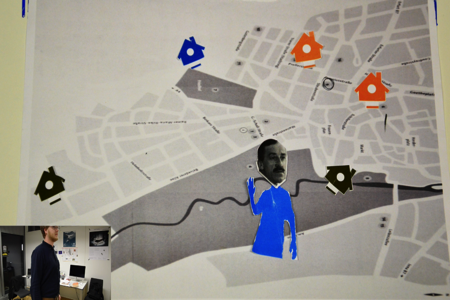
\includegraphics[width=\textwidth,height=6cm]{Figures/5/body_interaction}
        \caption{Body Interaction}
        \label{fig:body_inter_}
    \end{subfigure}
    \begin{subfigure}[H]{0.7\textwidth}
        \centering
        \includegraphics[width=\textwidth,height=6cm]{Figures/5/mobile_interactions}
        \caption{Mobile Interaction}
        \label{fig:mobile_inter}
    \end{subfigure}
    \caption{Bauhaus-Walk Advertisement Prototypes}
    \label{fig:Interactive_prototype}
\end{figure}

As can be seen in picture (A), the person in the left corner is physically walking and his blue silhouette in the screen is changing based on his location on the map. Picture (B) show Mobile interaction, in which the changes of the cursor in phone screen affects the movement of character on the map. To have a look at the entire paper prototype interaction sequences both for body and mobile, watch the prototype video\footnote{Ad Low-fi:\url{https://youtu.be/XGBgeSGeUwQ}, Last accessed 27th May 2016. } for all the process. \\


\section{Requirement gathering}
The below lists the \emph{Bauhaus-Walk} advertisement's functional and non-functional requirements. These requirements were the result of the focus-group and discussions.

\subsection{Functional Requirements}

\begin{enumerate}
\item	Detect multi User.
\item	Assign a character to the user. 
\item	Assign a task to the user.
\item	Respond to each user interaction.
\item	Show advertisement text.
\item	End the interaction.
\end{enumerate}


\subsection{Non-functional Requirements}

\begin{enumerate}
\item	Performance \\
This is a very important requirement that should be wisely done. Response time should be very fast in both gesture and mobile interaction so the user could see the reaction quickly on the screen. 

\item	Scalability \\
The interaction is scalable for multi-users at the same time for body interaction and mobile interaction.

\item	Availability \\
Kinect camera should be functional during the experiment for people detection, Access point should be running so that it could provide network access to users.

\item	Usability \\
The advertisement interaction both mobile and body should meet all criteria of usability.
\end{enumerate}

\subsection{Personas}
The below personas are created based on focus group findings since most people taking the tour are elder. The elder people build up my primary type of persona and young people build my secondary type persona as described below.


\begin{table}[H]
\centering
\caption{First persona}
\label{firstpersona}
\resizebox{8cm}{4cm}{ 
\begin{tabular}{l | l}
\tabhead{Type}   & Primary                             \\
\midrule
\tabhead{Name}            & Andreas Müller              \\
\midrule
\tabhead{Background}       & History teacher            \\
\midrule
\tabhead{Demographics}     & \begin{tabular}[c]{@{}l@{}}Age:.........................................50\\ Height:.....................................1,6 m\\ Martial status:.........................Married\\ Kids:........................................Two\\ Profession:................................School teacher\\ Language:.................................Deutsche\\ Computer experience:...............None\\ Smartphone experience:............None\end{tabular}                                                 \\
\midrule
\tabhead{Goal and Task} & \begin{tabular}[c]{@{}l@{}} \textbf{Experience goals:}\\ 1.Likes to learn about places in Weimar\\ 2.Likes to have fun.\\ 3.Does not like to feel alone and likes his wife or \\ friend to also join.\\ \textbf{End goals}\\ 1.Wants to see his body moving in the screen.\\ 2.Wants to explore the character’s location.\\ 3.Want to learn about Bauhaus-Walk program.\end{tabular} \\
\midrule
\tabhead{Environment}   & \begin{tabular}[c]{@{}l@{}}He and his friends want to learn about some good \\ places in Weimar and explore other famous culture events. \\ He does not use technology.\end{tabular}                                                                       
\end{tabular}
}
\end{table}



\begin{table}[H]
\centering
\caption{Second persona}
\label{secondpersona}
\resizebox{8cm}{4cm}{ 
\begin{tabular}{l | l}
\tabhead{Type}   & Secondary                             \\
\midrule
\tabhead{Name}            & Anna Weber              \\
\midrule
\tabhead{Background}       & Media art student            \\
\midrule
\tabhead{Demographics}     & \begin{tabular}[c]{@{}l@{}}Age:.........................................25\\ Height:.....................................1,6 m\\ Martial status:.........................Single\\ Kids:........................................None\\ Profession:................................Designer  \\ Language:.................................Deutsche, English, Spanish\\ Computer experience:...............Yes\\ Smartphone experience:............Yes\end{tabular}                                                 \\
\midrule
\tabhead{Goal and Task} & \begin{tabular}[c]{@{}l@{}} \textbf{Experience goals:}\\ 1.Avoid feeling stupid. \\ 2.Likes to try and error.\\ 3.Likes to have fun and laugh.\\ \textbf{End goals}\\ 1.To complete the task.\\ 2.Learn about Bauhaus-Walk program\\ \end{tabular} \\
\midrule
\tabhead{Environment}   & \begin{tabular}[c]{@{}l@{}}She is a student in Bauhaus University; she is very \\ interested in art and design and wants to find out more about \\ Weimar art. She loves using technologies \\like smartphone. \end{tabular}                                                                       
\end{tabular}
}
\end{table}



\section{Goal}
The goal of this evaluation is to find possible issues as listed below with interactive advertisement. 

\begin{enumerate}
\item   Confusing and unclear events or interactions.
\item   Misconception of a function.
\item   Task confusion.
\item   Understandability of advertisement goal and contents.
\end{enumerate}


\subsection{Questions}
The questions are divided for each individual interactions (mobile and body).

\subsubsection{Body Interaction}

\begin{itemize}
\item  Do users understand and react to the \emph{Call-to-Action} approach?
\item  Do users recognizes the character assigned to them?
\item  Do users understands the tasks assigned to them?
\item  Do users explore locations by moving their body in physical space?
\item  Do the prototypes raise alerts to specific user actions?
\item  Do the prototypes motivate participants to continue playing?
\end{itemize}

\subsection{Mobile Interaction}

\begin{itemize}
\item Do users understand the \emph{Call-to-Action} shown on the board?
\item Do users open the controller website by scanning QR-Code?
\item Does the Webpage prototype produce alerts with incorrect user input?
\item Do users rotate the mobile phone to start the game?
\item Do users understand the task?
\item Can users navigate the character by moving the face in mobile?
\item Does application produce alerts for incorrect location?
\end{itemize}


\section{Study Design}
\emph{Bauhaus-Walk} interactive prototypes consisted of two elements, (1) the screen that the users see the reaction of their action and advertisement content, (2) was the mean of interaction, body or mobile. To design the evaluation, the paper prototypes should be capable to mimic both of mentioned elements in real life scenario. Therefore I designed the actual advertisement screen paper prototype, in which the experimenter could simulate the output of all user action, even small actions like, movement of silhouette or character face on a display board that resembled a display.

\begin{figure}[H]
    \centering
    \begin{subfigure}[H]{0.48\textwidth}
        \centering
        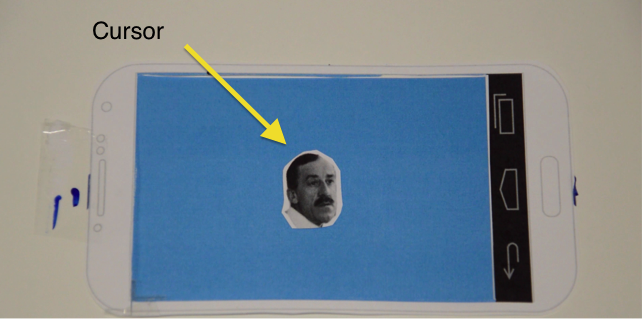
\includegraphics[width=\textwidth,height=5cm]{Figures/5/mobile_paper}
        \caption{Mobile paper prototype.}
        \label{fig:mobileproto}
    \end{subfigure}
    \begin{subfigure}[H]{0.48\textwidth}
        \centering
        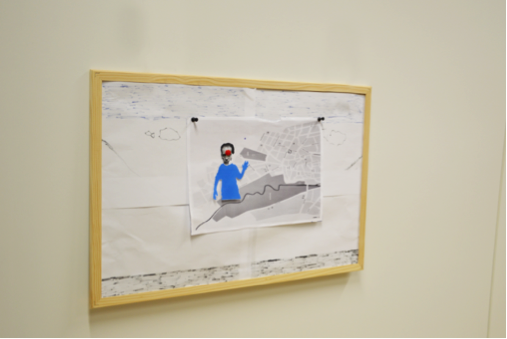
\includegraphics[width=\textwidth,height=5cm]{Figures/5/paper_board}
        \caption{Display board prototype.}
        \label{fig:screen_proto}
    \end{subfigure}
    \caption{Paper prototypes}
    \label{fig:paper_prototype_screen}
\end{figure}


\subsection{Subjects and location}
The prototype testing was limited to five participants, they were from different backgrounds, like Media Art, Media Architecture and Computer Science. Participants were invited to the Digital Bauhaus Lab ground floor.


\subsection{Procedures}

The below procedures were followed.

\begin{enumerate}
\item Participants were handed the information sheet and consent form for video recording.
\item Short introduction was given about the goal of the thesis and this evaluation in particular. But they were not given any clue about the interactive prototypes.
\item The task for participants, were to explore the paper prototype until the game gets finished and advertisement content is shown.
\item Participants interacted with both prototype one after another.
\item They were instructed to \emph{Think-Aloud} during the interaction to help the experimenter imitate the reactions on the board.
\end{enumerate}



\subsection{Display output simulation}
The moderator is a computer between display and a user, it would receive the user’s action by watching or listening to user and compute the result and show it on the display. All the interactive elements for the display were separately cut and put a side and each had a sticker at back. Whenever the user wanted to do something, for example visiting a location, the moderator would stick the picture of that place on display and also move the character based on the user’s physical movement.

\begin{figure}[H]
    \centering
    \begin{subfigure}[H]{0.48\textwidth}
        \centering
        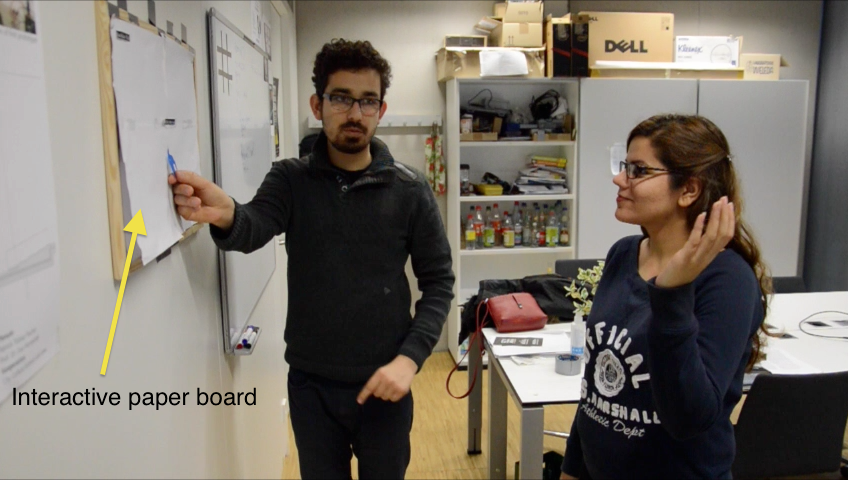
\includegraphics[width=\textwidth,height=5cm]{Figures/5/body}
        \caption{Participant interactig with body}
        \label{fig:screen_proto_inter}
    \end{subfigure}
    \begin{subfigure}[H]{0.48\textwidth}
        \centering
        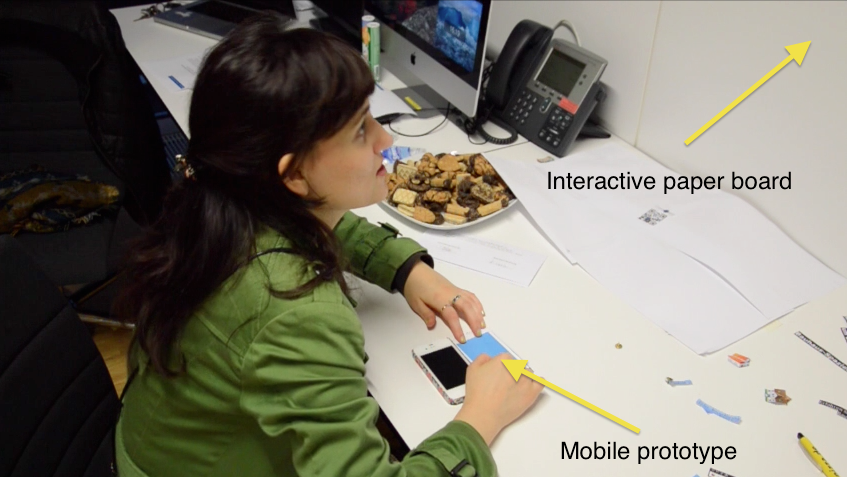
\includegraphics[width=\textwidth,height=5cm]{Figures/5/mobile}
        \caption{Participant interacting with mobile phone.}
        \label{fig:mobileproto_inter}
    \end{subfigure}
    \caption{Participants interactions}
    \label{fig:paper_prototype_screen}
\end{figure}

As it can be seen in picture (A), the user is interacting with her body and the moderator is holding the blue silhouette on the board and would change if user changed her position. The picture on the right shows the mobile interaction, the user is interacting with phone prototype and sees reaction in the display board. The display board cannot be seen in this picture frame.

\subsection{Data gathering}
The process of data gathering was as below. The methods were designed in a way to fully answer the research questions.


\begin{enumerate}
\item Video Recording \\
Each participant was video recorded for both body and mobile interactions for later observation and analysis purpose. 

\item Direct observation \\
Participants were observed during the interaction and users were also asked about what they thought at that moment while interacting. When participants could not perform a task then they were asked exploratory questions on how would they do the task naturally.

\item Think aloud \\
Participants were asked to read their mind while interacting with the prototypes. This helped to understand what they thought about a specific interaction at that moment. 

\item Interviews \\
After both paper prototype interactions were finished, a brief open-ended interview was taken to further learn about their experience with the prototypes. This interview was meant to get user comments and feedbacks for the prototypes. 


\begin{itemize}
\item What do you think about this technique?
\item Did you understand the blue person on the board?
\item What did you find difficult while interaction?
\item Did you understand that it was you but with different character?
\item What was confusing about this?
\item Do you like your face to be seen in public?
\item What needs to be changed?
\end{itemize}



\end{enumerate}




\section{Findings}
The important part for analyzing the data is shaped based on the defined hypothesis at the beginning; the below procedure was followed to best answer our open questions and to be able to evaluate both paper prototypes. 


All the interviews were transcribed one by one, and then thematic coding was applied to find common codes. For both prototypes four themes were focused while coding the interview transcripts, \emph{Likes, Dislikes, Confusing,} and \emph{User recommendations}. See Appendix see Appendix\ref{app:coded_interview} for the codes. Here I list all the usability issues that were extracted from direct observations and from Interview codings.


\subsection{Body Interactions}

\begin{enumerate}
\item Confusions 

\begin{enumerate}
\item  user was confused of how should the user walk, because it felt that there is not enough space. 
\item  User thought that if he/she moves to the location names or the icons, someone would guide her.
\item  User was confused on the new character photo labeled on the top of his silhouette; he thought that the new character is trying to interact with his silhouette. ``\emph{Is it like people approaching you and say hi and hello, and then ask me if I can visit his places}''
\item  User did not know his places (the character’s places).
\item  Could not understood the word move or walk, he taught that it is not applicable at the moment.
\item  Raise one hand to see if the blue reacts or not.
\item  Did not recognize the person.
\item  Did not understand the task partially.
\item  Did not understand what is the blue silhouette.

\end{enumerate}

\item Frustrations
\begin{enumerate}
\item  When the wrong house was explored, and she said ``\emph{(Ohh No)}''.
\item  Waiting for the houses to load on the screen.
\end{enumerate}

\item Mistakes
\begin{enumerate}
\item  Entered to the wrong location.
\item  Did not know how to navigate to the places. Although he was told that the silhouette is his body.
\item  Navigating the silhouette was a problem for her; she wanted to go on top of the map in the screen but physically moved back. And after seeing the reaction she corrected herself.
\end{enumerate}

\item Comments
\begin{enumerate}

\item   There should be very clear instruction in the application on what to do, what it is about and how to do it.
\item   I did not understand the person; maybe do not use it anymore.


\end{enumerate}
\end{enumerate}


\subsection{Mobile Interactions}
The below points lists all the possible issues with mobile interaction.

\begin{enumerate}

\item Confusions
\begin{enumerate}
\item  The idea of the application was not clear for her because she taught that the mobile application could be used when she goes out in the city. But later she found out that the screen and mobile are both of them used at a place.
\item  Navigation was a big confusion for him; he was touching the character on the mobile screen.
\item  The turning phone as shown in arrow, since she could not turn the phone.
\item  Did not understood what happened after the interaction was over. She did not read the texts or she did not understand why those were about.
\item  The face in the mobile.
\end{enumerate}

\item Frustrations
\begin{enumerate}
\item  Entering IP address.
\item  Visiting to all locations to finish the interaction.
\item  Not enough things when visiting to a location.
\item  She felt frustrated when visiting the wrong location and find the right location.
\item  He had to re-login because he accidently pressed cancel button.
\item  Visited to the wrong location.
\item  Waiting for the houses to load on the screen.
\end{enumerate}

\item Mistakes
\begin{enumerate}
\item  Did not understand to scan QR code.
\item  Took longer time to use the phone prototype. 
\item  Did not understand to rotate the mobile. As the instructions were shown on the phone.
\item  Took longer time to navigate the person on the screen.
\item  She tried to continue without putting any name in the form.
\item  Did not understand how to turn the phone, she touched the arrow on the screen many times. But nothing happened. Later she knew to turn the phone, but did not do it because she thought that the paper prototype should not be moved from its place.
\item  Could not navigate the person on the screen.
\item  Entered the wrong IP address, but then changed his mind and scanned the QR code.
\item  Accidently pressed cancel.
\end{enumerate}

\item Comments
\begin{enumerate}
\item  There is no enough information about the locations; it would be good to show a short description of the place.
\item  There could be like choices like when the opening time is for these locations.
\item  How far are they from my current location, the distance?
\item  View the transport possibilities to the selected locations.
\item  It would be good to have more information about the locations.
\item  And I would like to see the entire map on the phone too.
\item  I like to see some more information in my phone.
\item  There should be more guides when I use the phone, like there should be like Samsung, when you turn it on for the first time, it shows how to use what or it should have a finger picture to swipe on the face.
\end{enumerate}

\end{enumerate}

The below chart lists all the number of usability issues as, confusions, frustrations, and errors for each of the interactions carried by participants.

\begin{table}[H]
\caption{Number of usability issues}
\label{tab:prototypeusabilityissues}
\centering
\begin{tabular}{| l | c | c | c |}
\toprule
\tabhead{Prototype} & \tabhead{Confusion} & \tabhead{Frustration} & \tabhead{Errors} \\
\midrule
\textbf{Body}     & 9  &  2  &  3\\
\midrule
\textbf{Mobile}   & 5  &  7  &  9\\
\bottomrule
\end{tabular}
\end{table}

\subsection{Summary of findings}

This section summarizes the answers of this research questions based on above findings.

\subsubsection{Body Interaction}
\begin{itemize}
\item Do users understand and react to the \emph{Call-to-Action} approach? \\
\emph{Call-to-Action} of body prototype was ``\emph{To play come near!}''. All of the participants understood the it and reacted to it quickly as soon they read it.

\item Do users recognizes the character assigned to them?\\ 
All the participants did not understand the character, which was assigned to them. This happens when the participants do not have knowledge to know that character. It would be better to show a character that is very famous and is known to most of the population. Using very specific character is a bad idea. 

\item  Do users understands the tasks assigned to them?\\ 
Most users did not understand the task in the sense of the defined character, but they did understand that they should walk and explore locations.

\item Do users explore locations by moving their body in physical space? \\ 
As soon as users understood that the silhouette shown are theirs and then did the task by moving them selves physically, except one participant who did not understand until the observer gave him hint to move his self physically in right or left sides.

\item Do the prototypes raise alerts to specific user actions?   \\ 
The application did not raise error for user's specific interactions, for instance if the user was out of the screen or very close to the screen. Most of the participants raised their hands up, or turned around, there was no alerts for the participants.

\item Do the prototypes motivate participants to continue playing?\\ 
When the users explored the first location, they were excited and tried to see the other places too. All the actions were predictable by the participants and nothing new was happening, participants expected more from their interactions to be more excited to play the whole game. They did finish the game because they were told so.


\end{itemize}


\subsubsection {Mobile Interaction}
\begin{itemize}
\item Do users understand the \emph{Call-to-Action} shown on the board?\\ 
The participants were not shown the phone prototype at beginning, they were only shown the display only and were asked to react based on the messages or whatever they comprehend. After reading the \emph{Call-to-Action}, they asked for the phone prototype and then the phone prototype was shown to them to interact. 

\item Do users open the controller website by scanning QR-Code?\\ 
Four of the participants understood the use of QR-code and from which two of them scanned it and other two typed the IP address. One participant did not understood the use of QR-code.

\item Does the Webpage prototype produce alerts with incorrect user input?\\ 
The webpage did not produce error at many occasions while filling the form. It did not raise error when the cancel button was pressed, or when the game finished the application did not alert user to replay or leave webpage.

\item Do users rotate the mobile phone to start the game?\\ 
Only two of the participants rotated the phone but the rest of the participants tapped on the icon and tried to rotate the icon in the screen instead rotating the whole phone.

\item Do users understand the task?\\ 
This happened because all of the participants did not recognize the face and did not know where are his locations.

\item Can users navigate the character by moving the face in mobile?\\ 
Four of the participants touched and tapped the face shown on the mobile phone many times. They expected that something would happen after they touch the character like a dropdown list would appear to edit it, and one of the users dragged it and saw the reaction on the screen.

\item Does application produce alerts for incorrect location?\\ 
The incorrect locations that were explored by the participants were given an alert message.

\end{itemize}

\section{Conclusions}

Evaluation of low-fidelity prototype of \emph{Bauhaus-Walk} advertisement was very helpful. It exploited many design and interactions issues that could have been a bigger challenge if the problems were identified at the high fidelity version. This section concludes both body and mobile prototypes as below.

Firstly, the body prototype was easily understandable by most of the participants. The interaction was more natural and can be done by different kind of participant without having any technical expertise. Both of interactions in this technique \emph{Call-to-Action} and explore the locations were very natural and were performed faster. This low-fidelity usability testing suggested the changes needed for the next version of the advertisement i.e. the high - fidelity version. The changes would be to remove the character for users, improve alert messages for different user actions, enhance task description, and integrate features to increase interest of participants to be engaged with the advertisement.

Secondly, participants also appreciated the mobile interaction, but they were not so convinced for the usage because of many issues like logging onto web application, then navigating the face character. There were no clear instructions for how to navigate the character, and what would happen if there are many participants playing at the same time. It was unclear that what happens in web application when the interaction is over. This usability testing helped me to identify the mentioned usability problems and would help making changes for the new high fidelity version that would solve the current issues.

Thirdly, the advertisement text, which was shown at the end of interaction, did not catch the user's attention. It would be better to make a short video for the next prototype that would attract the user's attention on seeing the advertisement. After the video is over, the user continues to have his interaction to proceed with the application.

Finally, all usability related questions were taken in to account from which new decisions for the high fidelity version would be taken. The new version would overcome all the issues discovered until this stage. Participant’s recommendations and feedbacks had also much value and would be considered in the development phase.

